%%%%%%%%%%%%%%%%%%%%%%%%%%%%%%%%%%%%%%%%%%%%%%%%%%%%%%%%%%%%%%%%%%%%%%%%%%%%%%%%
% Needed and Layout
\documentclass[a4paper,11pt]{report}
\usepackage[utf8]{inputenc} % utf8 encoding
\usepackage{amsfonts}
\usepackage[T1]{fontenc} % use for allowing < and > in cleartext
\usepackage[margin=2.5cm]{geometry}

% Lists
\usepackage{verbatim}   % useful for program listings
\usepackage{enumitem}
\usepackage[ampersand]{easylist}

% Creating more compact lists
\let\olditemize\itemize
\renewcommand{\itemize}{
    \olditemize
    \setlength{\itemsep}{1pt}
    \setlength{\parskip}{0pt}
    \setlength{\parsep}{0pt}
}


% Creating my own inline code font
\newcommand{\textcode}[1]{
    \fboxsep=1pt
    \texttt{\colorbox{gray!20}{#1}}
}

% Recreating the figure thingy
\newcommand{\figa}{
    \begin{figure}[!htpb]
    \centering
}
\newcommand{\figb}[2]{
    \caption{#1}
    \label{#2}
    \end{figure}
}


% Math
\usepackage{mathtools}   % need for subequations
\usepackage{xfrac}       % Fractions  like 1/4 via \sfrac

% Graphics
\usepackage{graphicx}   % need for figures
\usepackage{color}      % use if color is used in text 
\usepackage{xcolor}     % use for text background color
\usepackage{tikz}
\usetikzlibrary{arrows}
\usepackage{float}

% Other
\usepackage{todonotes}
\usepackage{pdfpages}
\usepackage{subcaption}
\usepackage{latexsym}
\usepackage{fixltx2e}    % use for textsubscript
\usepackage[titletoc,title]{appendix}
\usepackage[framemethod=tikz]{mdframed}
\usepackage[titletoc,title]{appendix}
\usepackage{epstopdf}

% Code listing
\usepackage{listings} % For inserting code from file (I think)
\usepackage{algorithm}
\usepackage{algpseudocode}
\renewcommand{\algorithmicforall}{\textbf{for each}}
\makeatletter
\def\BState{\State\hskip-\ALG@thistlm}
\makeatother

\DeclareCaptionFormat{algor}{%
  \hrulefill\par\offinterlineskip\vskip1pt%
    \textbf{#1#2}#3\offinterlineskip\hrulefill}
\DeclareCaptionStyle{algori}{singlelinecheck=off,format=algor,labelsep=space}
\captionsetup[algorithm]{style=algori}

% URLs ? maybe
%\usepackage{hyperref}
\usepackage{url}
\usepackage[hypcap=false]{caption}


% for the \lstinputlisting for code blocks
\definecolor{codegreen}{rgb}{0,0.6,0}
\definecolor{codegray}{rgb}{0.5,0.5,0.5}
\definecolor{codepurple}{rgb}{0.58,0,0.82}
\definecolor{backcolour}{rgb}{1.0,1.0,1.0}
\lstdefinestyle{mystyle}{
  backgroundcolor=\color{backcolour},   
  commentstyle=\color{codegreen},
  keywordstyle=\color{magenta},
  numberstyle=\tiny\color{codegray},
  stringstyle=\color{codepurple},
  basicstyle=\ttfamily\footnotesize,
  breakatwhitespace=false,         
  breaklines=true,                 
  captionpos=b,                    
  keepspaces=true,                 
  numbers=left,                    
  numbersep=1pt,                  
  showspaces=false,                
  showstringspaces=false,
  showtabs=false,                  
  tabsize=2
}
\lstset{style=mystyle}

\begin{document}

% Configuration
\setlength{\parindent}{0cm}
\setlength{\unitlength}{1mm}

% Front Page
\date{September 1st 2015\\ IT University of Copenhagen}
\title{A Quantitative Analysis of Variability Bugs in Linux}
\author{Elvis Flesborg\\
\texttt{efle@itu.dk}}
\clearpage\maketitle
\thispagestyle{empty}
\newpage

%%%%%%%%%%%%%%%%%%%%%%%%%%%%%%%%%%%%%%%%%%%%%%%%%%%%%%%%%%%%%%%%%%%%%%%%%%%%%%%%
%                           TABLE OF CONTENTS
%%%%%%%%%%%%%%%%%%%%%%%%%%%%%%%%%%%%%%%%%%%%%%%%%%%%%%%%%%%%%%%%%%%%%%%%%%%%%%%%
\tableofcontents
\thispagestyle{empty}



\newpage

\setcounter{page}{1}

\chapter{Abstract}
\emph{---Leave blank until the end---}

\chapter{Introduction}
\emph{---Leave blank until the end---}


% TODO
\begin{itemize}
    \item \underline{\textbf{TODO}}
        \item Explain about representative samples
\end{itemize}


%%%%%%%%%%%%%%%%%%%%%%%%%%%%%%%%%%%%%%%%%%%%%%%%%%%%%%%%%%%%%%%%%%%%%%%%%%%%%%%%
%                           BACKGROUND
%%%%%%%%%%%%%%%%%%%%%%%%%%%%%%%%%%%%%%%%%%%%%%%%%%%%%%%%%%%%%%%%%%%%%%%%%%%%%%%%
\newpage
        \chapter{Background}

A \emph{Linux} operating system is often referring to a a \emph{GNU/Linux} 
operating system, where the Linux part of \emph{GNU/Linux} is the Linux kernel, 
and the \emph{GNU} part is a software bundle with utilities (eg. a shell, a 
compiler, etc...) \cite{gnu_pack}. Both is 
needed, to have a working operating system. 
\\

This report will only focus on the \emph{Linux kernel}, and not the \emph{GNU} 
bundle.


        \section{The Linux Kernel and Variability}


Many software products are configurable in some way. This creates the 
possibility of tailoring the software to suit different needs. For example 
different kinds of hardware, or different functionalities. This is called 
\emph{variability} in software or \emph{Software Product Lines} (SPL), when 
different programs can be made from the same source code base.
    \footnote{Check definition of SPL, and write it here}

The options that can be changed, are called \emph{features}.
\\

The Linux kernel is very configurable. In the configuration files (the Kconfig 
files), there is a total of 14,387 different features, that can be configured.
    \footnote {14,387 across all architectures, with an average of 9,984 per 
        architecture}
It is the open source software product with the highest degree of variability.

This high degree of variability has also had an impact on the use cases for the 
Linux kernel. Linux is used for anything from small embedded devices (like car 
GPSs, and cell phones) to supercomputers.
In fact 98\% of the top 500 supercomputers in the world run a Linux distibution
    \cite{top500}
.
\\

This high variability rate makes maintaining the code somewhat harder to 
grasp, and this makes the code base more error prone. So what you get in 
scalability you pay for in complexity of maintaining the code. 
    \footnote{Refer to Jean's project or something}
    \footnote{Also refer to a paper that andrjew made about industrial 
        something. It said something about how much more efficient the code was,
        when variability was there.}


        \section{Linux Kernel Development}

\begin{center}
    \emph{
        Comment from the linux-next page or something
    }
\end{center}


        \subsection{Mainline tree}

The Linux kernel development cycle has approximately 2$\sfrac{3}{4}$ months 
from one stable release to the next stable release
    \cite{crystalball}
.
In the meantime, \emph{RC} 
releases, also called \emph{prepatch} releases, are released once in a while. 
Mainly for kernel developers to test for new features. 


        \subsection{Stable trees}

Then, when the top maintainers of the mainline tree think that the kernel is 
stable enough, a new stable version is created, and the whole process is 
repeated.


        \subsection{linux-next tree}

Then there is the \emph{linux-next} tree. It is a \emph{git} repository, which 
merges over 200 other \emph{git} repositories
    \footnote{See <src>/Next/Trees}
, which 
are all based on the \emph{mainline} tree. The \emph{linux-next} tree is 
merging these other trees every day and the merge conflicts are handled. 
Therefore the \emph{linux-next} tree always contain the newest commits. 

This tree will get some bugs fixed sooner than if everyone contributed to the 
mainline and tested on that. Comparing to a stable version, one would suspect 
the \emph{linux-next} tree to have more bugs, since it has not been tested, 
and it is the newest code available, which means more bugs have been inserted. 

This leads to our first research question.
\\

\textbf{RQ1:} Will the unstable linux-next repository generate more errors than 
the stable kernel.
\\

For this thesis project, both the \emph{linux-next} tree and the latest stable 
version is used. As time of data gathering, the latest stable version is 
\emph{4.1.1}.

    \footnote{http://neuling.org/linux-next-size.html}
    \footnote{http://news.gmane.org/gmane.linux.kernel.next - the linux-next 
        mailing list archive}
    \footnote{http://kisskb.ellerman.id.au/kisskb/matrix/ - this is some kind of
        build robot results page.}
    \footnote{
        http://git.kernel.org/cgit/linux/kernel/git/next/linux-next.git/
        tree/Next/Trees ?id=HEAD - here are all the git trees that are merged 
        in linux-next}


        \section{Inner Workings of Linux Kernel}

This section will explain in coarse detail, the structure of the Linux kernel.
From the directory structure, over configuration, to compilation of the kernel.


        \subsection{Subsystems}

The directories in the root folder of the Linux kernel source code are called 
\emph{subsystems}. 

% --- Not showing this graph ---
% \figa
%     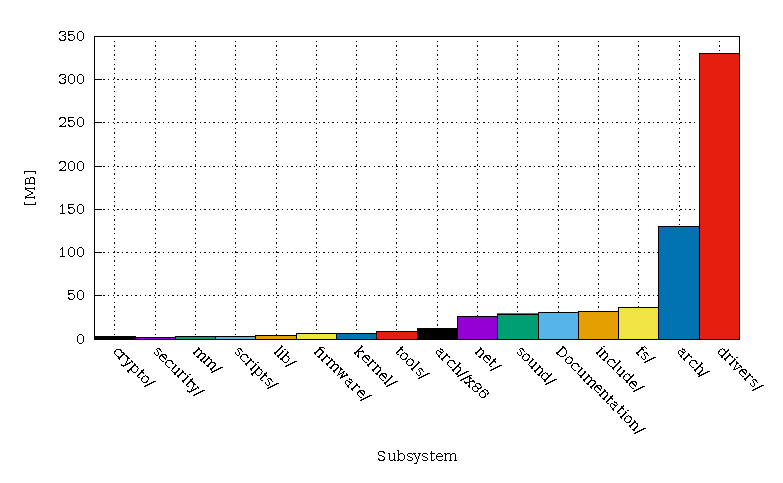
\includegraphics{plots/subsystemsizes.eps}
% \figb{Visualization of the sizes of the subsystems}{fig:subsystems}
% ---

The \textcode{drivers/} subsystem is by far the largest subsystem. It contains 
all hardware drivers. It is also mostly contributed to by hardware vendors.
    \footnote{Source? and is it true? -What would Greg Kroah Hartman say?}
Since it is the largest subsystem, one could suspect it to contain the most 
errors. And even when taking relative size into account, one could suspect this
on the grounds of the majority of the code being written by hardware vendors.

This leads to next research question:

\textbf{RQ2:} In what subsystems do the most errors occur. And in the largest 
subsystems, in what subsubsystem? 
\\


The \textcode{arch/} contains architecture specific source code. In this project, 
only the \textcode{arch/x86} architecture is compiled for, so only this 
subsubsystem will be in use. 

Many of these architectures are very rarely used in day to day computing, but 
they are one of the reasons that Linux can run on so many devices. There are 30 
architectures in the \textcode{arch} folder.

% --- Not showing this graph ---
% \figa
%     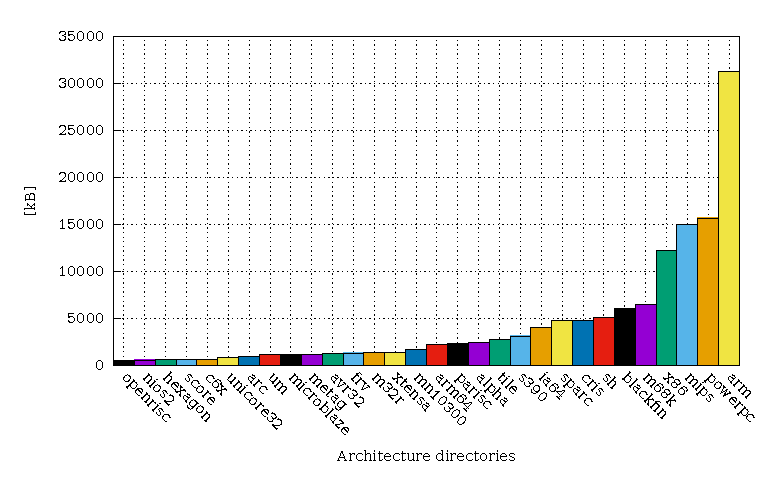
\includegraphics{plots/archsizes.eps}
% \figb{The sizes of the different architecture diretories}{fig:archsizes}
% ---


% TODO
\begin{itemize}
    \item \underline{\textbf{TODO}}
    \item Find out how to find the exact number of possible configurations. It 
        is in some article, I got by Andrzej. Plus maybe SharpSAT.
    \item Explain how to find the number of features by grepping.
    \item Talk about subsystems
    \item Maybe talk about the percentage of code in every subsystems. What is 
        Linux kernel made of?
    \item talk about who contributes to the kernel. (intel, novell). Both in 
        code and money?
    \item mention some more subsystems other than drivers and arch
\end{itemize}


\subsection{Kconfig - The Feature Model Language}

\paragraph{A feature model} is a way of representing all the possible 
configurations - \emph{the configuration space}. 

that describes the feature model of the Linux kernel.
It contains dependencies and 
constraints for the features, and if a chosen configuration fulfills the 
constraints, then the configuration is valid.

For a given configuration $\kappa$, it must satisfy the feature model 
$\psi_{FM}$.

\begin{equation}
    \kappa \in \psi_{FM}
\end{equation}

\paragraph{The Kconfig language} is the language of the feature model in Linux 
(also used for other projects like busybox, buildroot, and others).
    \footnote{Cite the Variablity Modeling in the systems software domain paper}
The configuration files have the prefix \textcode{Kconfig}, and are 
scattered all over the Linux kernel source code tree, where they include each 
other.
\\

The different data types are \textcode{boolean}, \textcode{tristate}, 
\textcode{string}, \textcode{hex}, and \textcode{integer}.

See figure ~\ref{kconfigchoice} and figure ~\ref{kconfigtypes} for some real 
example of the Kconfig syntax. Figure ~\ref{kconfigchoice} shows an example of 
a \textcode{choice} option, where only one of multiple features 
can be enabled. 

\figa
    \lstinputlisting[language=C, firstline=1, morekeywords={prompt, config, 
        depends, on, bool, endchoice, choice,{||}}]{code/kconfigtypesreal}
\figb{A real Kconfig example showing the basic data types}{kconfigchoice}

\figa
    \lstinputlisting[language=C, firstline=1, morekeywords={prompt, config, 
        depends, on, bool, endchoice, choice,{||}}]{code/kconfigboolreal}
\figb{A real Kconfig example showing a choice clause with 5 
    choices}{kconfigtypes}

\figa
    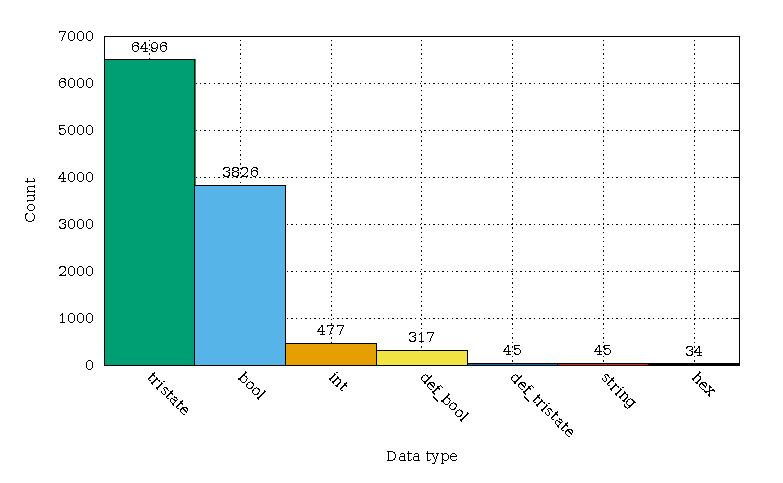
\includegraphics{plots/datatypestats.eps}
\figb{The distribution of different datatypes in the feature 
    model}{datatypesdistribution}

This can be visualized in feature diagram. The example will be tiny compared to 
that of the Linux kernel. The feature model of the Linux kernel is too big 
to fit in a normal sizes report.

See figure ~\ref{featurediagramcar} for the toy example of a feature 
diagram. It depicts a feature model of a car configuration, where there are 
some mandatory features and some optional, and also a choice option for the 
transmission. A cross-tree dependency is also present.

% 65 lines down to \figb
\figa
    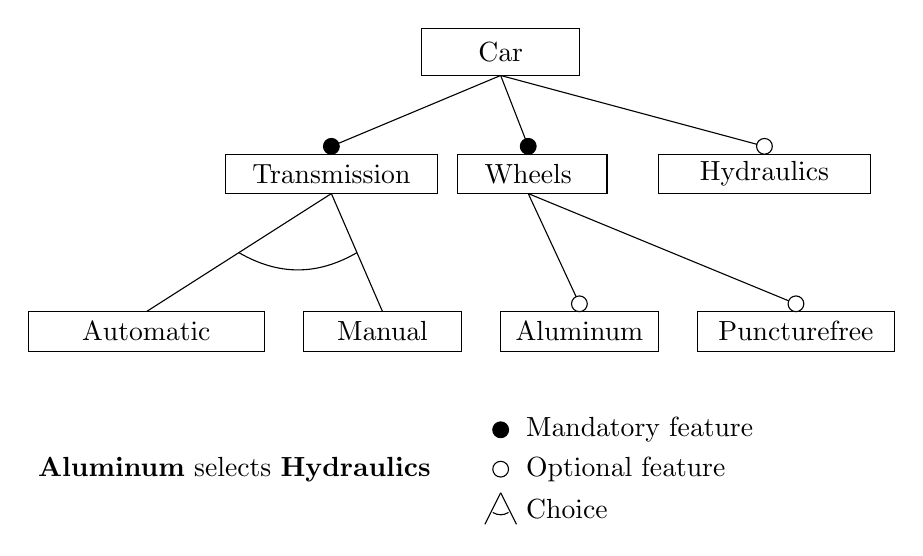
\begin{tikzpicture}
        % The top box
        \draw (2,3) rectangle (4,3.6);
        \draw (3,3.3) node {Car};

        % The other boxes
        \draw (-0.5,2) rectangle (2.2,1.5);
        \draw (2.45,2) rectangle (4.35,1.5);
        \draw (5,2) rectangle (7.7,1.5);

        \draw (-3,0) rectangle (0,-0.5);
        \draw (0.5,0) rectangle (2.5,-0.5);
        \draw (3,0) rectangle (5,-0.5);
        \draw (5.5,0) rectangle (8,-0.5);

        % The words in the boxes
        \draw (0.85,1.75) node {Transmission};
        \draw (3.35,1.75) node {Wheels};
        \draw (6.35,1.75) node {Hydraulics};

        \draw (-1.5,-0.25) node {Automatic};
        \draw (1.5,-0.25) node {Manual};
        \draw (4,-0.25) node {Aluminum};
        \draw (6.75,-0.25) node {Puncturefree};

        % The edges
        \draw (0.85,2.1) edge (3,3);
        \draw (3.35,2.1) edge (3,3);
        \draw (6.35,2.1) edge (3,3);

        \draw (-1.5,0) edge  (0.85,1.5);
        \draw (1.5,0) edge  (0.85,1.5);
        \draw (4,0.1) edge  (3.35,1.5);
        \draw (6.75,0.1) edge  (3.35,1.5);

        % The 'or'
        \draw (-0.325,0.75) edge [bend right] (1.175,0.75);

        % The dots
        \draw[fill=black] (0.85,2.1) circle (0.1);
        \draw[fill=black] (3.35,2.1) circle (0.1);
        \draw[fill=white] (6.35,2.1) circle (0.1);

        \draw[fill=white] (4,0.1) circle (0.1);
        \draw[fill=white] (6.75,0.1) circle (0.1);

        % The legend
        \draw[fill=black] (3,-1.5) circle (0.1);
        \draw[fill=white] (3,-2) circle (0.1);
        \draw[right] (3.2,-1.5) node {Mandatory feature};
        \draw[right] (3.2,-2) node {Optional feature};

        \draw (3.0,-2.3) edge (3.2,-2.7);
        \draw (3.0,-2.3) edge (2.8,-2.7);
        \draw (3.1,-2.55) edge [bend left] (2.9,-2.55);
        \draw[right] (3.2,-2.5) node {Choice};

        % The cross-tree dependency
        \draw[right] (-3, -2) node {\textbf{Aluminum} selects 
            \textbf{Hydraulics}};

    \end{tikzpicture}
\figb{An example of a feature diagram of a car}{featurediagramcar}
% 65 lines up to \figa

\begin{itemize}
    \item \underline{\textbf{TODO}}
    \item Explain what the Linux kernel tree is.
    \item Find another example than a car
    \item Find a more simple Kconfig code example
    \item It creates a `.config` file.
    \item Explain the Kconfig language a bit
    \item Examples of constraints in the language
    \item Reference to Thorsten's projects
    \item Refer to the /Documentation/kbuild/kconfig-language.txt
    \item explain that CONFIG\_MMU and MMU is the same
    \item Should I have the Backus Naur Form of the Kconfig language here?
\end{itemize}

\subsection{randconfig}

The Linux kernel comes with different ways of creating your own configuration 
file. There is a question based one (\emph{config}), and some menu based ones 
(\emph{menuconfig}, \emph{xconfig}, \emph{nconfig}, \emph{gconfig}), but also 
some that will never prompt the user for anything, but create some automated 
config (\emph{allyesconfig}, \emph{allnoconfig}, \emph{defconfig}, and 
\emph{randconfig}).
\\

That last one \emph{randconfig} is interesting, as it will go through the 
Kconfig feature model files, and pick random values for all of the features. 
This should be perfect for the goal for this project. Although time will tell 
that it is indeed biased, and will not create configurations that are of 
representative character. 

See figure ~\ref{randconfigtoy} for a toy example of a Kconfig feature model. 
It is a very small example with only two features, but it will easily explain 
some limitations of \emph{randconfig}.

\figa
    \lstinputlisting[language=C, firstline=1, morekeywords={prompt, config, 
        depends, on, bool, endchoice, choice,{||}}]{code/kconfigrandconfigtoy}
\figb{A toy Kconfig feature model}{randconfigtoy}


\figa
    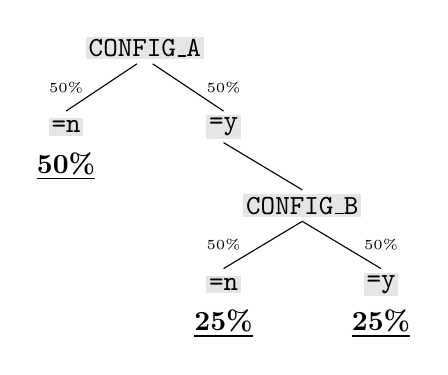
\begin{tikzpicture}
        % Names of configs
        \draw (2,4) node {\textcode{CONFIG\_A}};
        \draw (4,2) node {\textcode{CONFIG\_B}};

        % yeses and nos
        \draw (1,3) node {\textcode{=n}};
        \draw (3,3) node {\textcode{=y}};
        \draw (3,1) node {\textcode{=n}};
        \draw (5,1) node {\textcode{=y}};

        % lines not necessarily from above and down
        \draw[-] (1.9,3.8) edge (1,3.2);
        \draw[-] (2.1,3.8) edge (3,3.2);
        \draw[-] (3,2.8) edge (4,2.2);
        \draw[-] (3,1.2) edge (4,1.8);
        \draw[-] (5,1.2) edge (4,1.8);

        % Draw percentages
        \draw (1,3.5) node {\tiny{50\%}};
        \draw (3,3.5) node {\tiny{50\%}};
        \draw (3,1.5) node {\tiny{50\%}};
        \draw (5,1.5) node {\tiny{50\%}};

        \draw (1,2.5) node {\textbf{\underline{50\%}}};
        \draw (3,0.5) node {\textbf{\underline{25\%}}};
        \draw (5,0.5) node {\textbf{\underline{25\%}}};

    \end{tikzpicture}
\figb{A toy example showing the way randconfig selection of 
    features}{randconfigtoy50}

In the example in figure ~\ref{randconfigtoy50} shows that the three possible 
configurations (\textcode{\{\}}, \textcode{\{A\}}, and \textcode{\{A,B\}}) do 
not have the same chance of getting created by \emph{randconfig}.

For the creation to be representative, all the three possible configurations 
should have equal chance of being created (33\%). See figure 
~\ref{randconfigtoy33} for a visualization of how the selection should be to be 
representative.

\figa
    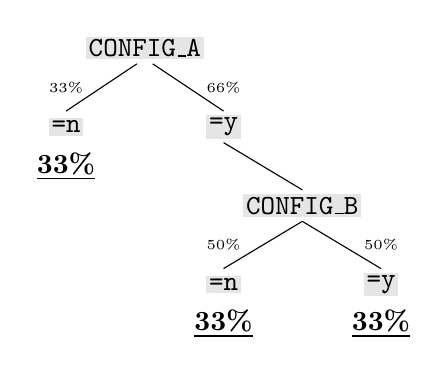
\begin{tikzpicture}
        % Names of configs
        \draw (2,4) node {\textcode{CONFIG\_A}};
        \draw (4,2) node {\textcode{CONFIG\_B}};

        % yeses and nos
        \draw (1,3) node {\textcode{=n}};
        \draw (3,3) node {\textcode{=y}};
        \draw (3,1) node {\textcode{=n}};
        \draw (5,1) node {\textcode{=y}};

        % lines not necessarily from above and down
        \draw[-] (1.9,3.8) edge (1,3.2);
        \draw[-] (2.1,3.8) edge (3,3.2);
        \draw[-] (3,2.8) edge (4,2.2);
        \draw[-] (3,1.2) edge (4,1.8);
        \draw[-] (5,1.2) edge (4,1.8);

        % Draw percentages
        \draw (1,3.5) node {\tiny{33\%}};
        \draw (3,3.5) node {\tiny{66\%}};
        \draw (3,1.5) node {\tiny{50\%}};
        \draw (5,1.5) node {\tiny{50\%}};

        \draw (1,2.5) node {\textbf{\underline{33\%}}};
        \draw (3,0.5) node {\textbf{\underline{33\%}}};
        \draw (5,0.5) node {\textbf{\underline{33\%}}};

    \end{tikzpicture}
\figb{A toy example showing a correct selection of features}{randconfigtoy33}

This has apparently not been implemented in the Linux kernel tools, because 
representativeness does not matter for what it is used for. It is merely used 
as a simple testing tool.

To make this representative, one would have to make \emph{randconfig} aware of 
the whole dependency tree or the whole configuration space before randomly 
selecting, to skew the possibilities. This seems infeasible since the 
configuration space is so large.
\\

Some different ways of generating a representative sample was considered. In 
the end, \emph{randconfig} was chosen because it showed to be too cumbersome to 
create a method that actually was representative. 

The methods that was considered will be explained later in this report. 
    \footnote{refer to it when you have written it} 
They included the aforementioned \emph{randconfig} tool being rewritten, a 
script that scrambled the Kconfig files, and a generate and filter method.
\\



% TODO
\begin{itemize}
    \item \underline{\textbf{TODO}}
    \item Show some code of randconfig not doing it representatively
    \item show results from running randconfig a 1000 times.
    \item Talk about how there is 7 layers of dependencies. And how I found out.
    \item \^ Hmm . Are there only 7 layers when counting ifs? what about 
        'depends on's
    \item show some scrots of menuconfig/allnoconfig/gconfig
    \item mention that it is also called a preprocessor.
\end{itemize}


\subsection{Compilation}

When a configuration has been created, the Linux kernel is compiled using 
that configuration file. This is done mainly by \emph{gcc - The GNU Compiler 
Collection}, which then outputs warning and error 
messages. If there is an error, the compilation will also stop immediately 
(sometimes it will try to keep on going, but in this project, it is told to 
stop after one error).

These output messages hold the information that will be used in this project. 
In a warning, there is information about a possible coding mistake that might 
break the code. There are about 30 different warning types \cite{gccwarnings}
Some of these are not so interesting as others for this project.\\


Generally there will be distinguished between four different types of output. 
These are \emph{relevant errors}, \emph{irrelevant errors}, \emph{relevant 
warnings}, and \emph{irrelevant warnings}. 


\paragraph{The relevant errors} 
are reproducible errors that will occur on all 
machines when a certain configuration is being built. 
    \footnote{Refer to the list of errors - some link somewhere}

\paragraph{The irrelevant errors} 
are a result of the building system not having some specific dependencies 
installed.
\\

For instance, there is a feature in the feature model that is called 
\textcode{CONFIG\_KERNEL\_LZO}, which dictates that the kernel should be 
compressed by the \emph{lzop} library instead of the default \emph{gzip} 
compression library.

If a configuration has the \textcode{CONFIG\_KERNEL\_LZO} enabled, then to 
build the kernel, the \emph{lzop} library will have to be installed on the 
build system. If it is not, then the compilation will stop with an error.

There are six different ways to compress the Linux kernel (\emph{gzip}, 
\emph{bzip2}, \emph{lzma}, \emph{xz}, \emph{lzo}, and \emph{lz4}),
    \footnote{refer to the picture of gconfig and friends}
which leads to that every sixth compilation will stop with the same error.
\\

There exist many other examples like this in the \emph{Linux kernel} where an 
uninstalled program will result in an unbuilt kernel. These \emph{irrelevant 
errors} would have to be minimized, since they are not actual kernel errors, 
but local errors. 
    \footnote{Give list of all the features I have disabled} 

On the build system for this project, the \emph{lzo} package was in the Linux 
distribution's repository, and therefore easy to install. The \emph{lz4} 
packager however was not.
\\

The following list is a \emph{build system mandatory features}
    \footnote{maybe find another word for this?}
list, which decreases the configuration space of this project, but otherwise 
would just give a lot of false positives.

All these lines are added to the configurations, which are generated in
this project.

\begin{itemize}
    \item \textcode{CONFIG\_STANDALONE=y}
    \item \textcode{CONFIG\_FW\_LOADER=n}
    \item \textcode{CONFIG\_SECCOMP=y}
    \item \textcode{CONFIG\_PREVENT\_FIRMWARE\_BUILD=y}
    \item \textcode{CONFIG\_*LZ4*=n}
        \footnote{This means that all features having to do with \emph{lz4} 
                    were disabled}
\end{itemize}

See chapter~\ref{sec:ttv} about Threats to Validity on page \pageref{sec:ttv} 
for a more thorough description of the specific features.


\paragraph{The relevant warnings}
are warnings that may cause an error at some point. The \emph{uninitialized 
variable} warning is such a warning. If a variable is uninitialized, and ends 
up being called, it may cause an error, and stop the compilation. See figure 
~\ref{lst:uninitvar} for a code example.

The relevant warnings are:

\begin{itemize}
    \item Uninitialized variable
    \item Maybe uninitialized
    \item Overflow
    \item Deprecated declarations
        \footnote{Complete this list}
\end{itemize}

\figa
    \lstinputlisting[language=C, firstline=3]{code/uninitvar.c}
\figb{A toy program showing an uninitialized variable.}{lst:uninitvar}

The program in figure ~\ref{lst:uninitvar} will return the warning 
'\texttt{'a' is used uninitialized in this function [-Wuninitialized]}' and the 
output, when the program is run, will be '\texttt{0Hello world}'.

\paragraph{The irrelevant warnings}
These are mainly warnings that represent dead code. Warnings like \emph{unused 
function}, \emph{unused variable}, \emph{unused label}, and \emph{unused 
value}, will all end up as dead code, which is bad for fitting a kernel 
on some hardware with limited space. Apart from that it is nothing else than 
code pollution. See figure ~\ref{lst:unusedvar} for a code example  of an 
unused variable.

The irrelevant warnings are:

\begin{itemize}
    \item Unused function
    \item Unused variable
    \item Unused label
    \item Unused value
        \footnote{Complete this list}
\end{itemize}

\figa
    \lstinputlisting[language=C, firstline=3]{code/unusedvar.c}
\figb{A program resulting in an unused variable warning.}{lst:unusedvar}

This will return the warning '\texttt{unused variable 'a' [-Wunused-variable]}'.

% TODO
\begin{itemize}
    \item \underline{\textbf{TODO}}
    \item Give real examples of unused function, and uninitialed... MAYBE
\end{itemize}


%%%%%%%%%%%%%%%%%%%%%%%%%%%%%%%%%%%%%%%%%%%%%%%%%%%%%%%%%%%%%%%%%%%%%%%%%%%%%%%%
%                           METHODOLOGY
%%%%%%%%%%%%%%%%%%%%%%%%%%%%%%%%%%%%%%%%%%%%%%%%%%%%%%%%%%%%%%%%%%%%%%%%%%%%%%%%
\newpage
\chapter{Methodology}

The objective is to make a quantitative analysis of errors and warnings in the 
Linux kernel based on as many random configurations as are possible to generate 
within the time span of this project.

There will be generated random configurations, and these will be used to 
compile two Linux kernels. One stable Linux kernel, and one from the 
linux-next repository.  
\\


\section{Research Questions}


It is likely that some errors or warnings are more severe than others, and some 
types of errors get fixed more than others. This leads to the next question.
\\


\textbf{RQ2:} What warnings are mostly generated.  
\\


And this can also be different between the stable and unstable versions. Hence 
the next question. 
\\


\textbf{RQ3:} What bugs seem to be fixed the most when going from unstable to 
stable. 
\\


As mentioned \footnote{Where is this mentioned about the subsystems? refer to 
it}, the subsystems of the kernel are of very different character. 
\footnote{mention somewhere earlier, that drivers are different from security 
or kernel} And therefore the bug types must differ from subsystem to subsystem. 
\\




\textbf{RQ5:} What percentage of the possible configurations for the Kernel are 
valid. 
\\


\textbf{RQ6:} Are there any specific features, that when enabled, will produce 
more warnings than others. 
\\




\section{Collecting data}

Every time a randomly configured compilation is running, \emph{gcc} will 
output warning and error messages in the \emph{standard error} output. This 
output is then scraped through to categorize it.

An output line will contain a \emph{bug type}, a \emph{filename}, \emph{line 
number}, and a \emph{message} describing the warning in english.


The collection of data has mainly been done on a computer at the IT University 
of Copenhagen. It has 32 cores and 128 GB of RAM, and the mean time to compile 
a kernel and upload the data was around 1 minute and 35 seconds. A fairly 
regular laptop with 4 cores and 8 GB of RAM does that in just over 8 minutes 
on average. 
\\


When a compilation is done, the output is scraped and categorized, and then 
uploaded to a database, for easy querying during and after the project. 

See the figures ~\ref{fig:conftable}, ~\ref{fig:bugstable}, and 
~\ref{fig:filestable} for the database tables.


\figa
    \begin{tabular}{c|c|c}
        \hline 
        \hline
        \multicolumn{3}{c}{\textbf{Configurations}} \\
        \hline
        \textbf{Name} & \textbf{Type} &\textbf{primary key} \\
        \hline
        hash & char(64) & primary key \\
        exit\_status & int(1) \\
        conf\_errs & text \\
        linux\_version & varchar(100) & primary key \\
        original & longtext \\
        \hline
        \hline
    \end{tabular}
\figb{The Configurations table}{fig:conftable}

\figa
    \begin{tabular}{c|c|c}
        \hline
        \hline
        \multicolumn{3}{c}{\textbf{Bugs}} \\
        \hline
        \textbf{Name} & \textbf{Type} &\textbf{primary key} \\
        \hline
        hash & char(64) & primary key \\
        type & varchar(50) \\
        linux\_version & varchar(100) \\
        config\_hash & char(64) \\
        subsystem & varchar(30) \\
        original & longtext \\
        \hline
        \hline
    \end{tabular}
\figb{The Bugs table referring to the Configurations table}{fig:bugstable}

\figa
    \begin{tabular}{c|c|c}
        \hline
        \hline
        \multicolumn{3}{c}{\textbf{Files}} \\
        \hline
        \textbf{Name} & \textbf{Type} &\textbf{primary key} \\
        \hline
        id & int(11) & primary key \\
        path & varchar(50) \\
        line & varchar(15) \\
        bug\_id & char(64) \\
        \hline
        \hline
    \end{tabular}
\figb{The Files table referring to the Bugs table}{fig:filestable}

% TODO
\begin{itemize}
    %\item Grepping the stderr
    \item Tell why we need to compile
    \item Tell about coccinelle, and why we dont use that
    \item Categorizing the warnings/Errors
    %\item About the collection machine
    %\item About the database setup
\end{itemize}




%%%%%%%%%%%%%%%%%%%%%%%%%%%%%%%%%%%%%%%%%%%%%%%%%%%%%%%%%%%%%%%%%%%%%%%%%%%%%%%%
%                                 DATA
%%%%%%%%%%%%%%%%%%%%%%%%%%%%%%%%%%%%%%%%%%%%%%%%%%%%%%%%%%%%%%%%%%%%%%%%%%%%%%%%
\newpage
\chapter{Data}

%\begin{itemize}
    %\item Example of data structure
    %\item Graph of tables
%\end{itemize}



% TODO
\begin{itemize}
    \item \underline{\textbf{TODO}}
        \item 
\end{itemize}

%%%%%%%%%%%%%%%%%%%%%%%%%%%%%%%%%%%%%%%%%%%%%%%%%%%%%%%%%%%%%%%%%%%%%%%%%%%%%%%%
%                               RESULTS
%%%%%%%%%%%%%%%%%%%%%%%%%%%%%%%%%%%%%%%%%%%%%%%%%%%%%%%%%%%%%%%%%%%%%%%%%%%%%%%%
\newpage
\chapter{Results}

\section{Analyzing the data}

\section{Number of valid configurations}

\section{Observations}


% TODO
\begin{itemize}
    \item \underline{\textbf{TODO}}
        \item 
\end{itemize}


%%%%%%%%%%%%%%%%%%%%%%%%%%%%%%%%%%%%%%%%%%%%%%%%%%%%%%%%%%%%%%%%%%%%%%%%%%%%%%%%
%                           THREATS TO VALIDITY
%%%%%%%%%%%%%%%%%%%%%%%%%%%%%%%%%%%%%%%%%%%%%%%%%%%%%%%%%%%%%%%%%%%%%%%%%%%%%%%%
\newpage
\chapter{Threats to Validity}
\label{sec:ttv}



\section{Generalization}

One major threat to validity is in the representativeness of the random 
configurations. Since the configurations are created using the \textcode{make 
randconfig} method, some configurations are more likely to be generated than 
others.

This means, that when something is generally said about all of the Linux 
Kernel, instead something is said about mostly a subset of Linuxes. See figure 
~\ref{fig:repsubset} for a subset of configurations, where generalization is 
representative, and figure ~\ref{fig:unrepsubset} for the opposite.

\figa
    \emph{Show an image of true representativeness}
\figb{A representative subset}{fig:repsubset}

\figa
    \emph{Show an image of true representativeness}
\figb{A representative subset}{fig:unrepsubset}

Another idea was to take all the spread out Kconfig files, and concatenate 
them all into one big text file, which would then be modified. If the order of 
the features were randomized, then the coins would not be flipped in the same 
order every time, and this could have an effect on the dependent features. \\

The third idea was to manually generate a configuration file, and then check - 
somehow - if the config file was valid, and then use it if it was valid. By 
not looking at dependencies, but only considering \emph{choice} options and 
enabling \emph{mandatory features}, a configuration file was created by 
randomly flipping a coin per each feature.

This seemed doable until after generating 100,000 configurations, not one 
valid configuration was found. It seems like many of the $2^{11,000}$ 
configurations are invalid.

\subsection{Architecture}

To create a true representative sample space, all the different architectures 
should be compiled for. There exist 31 different architectures, but the most 
common one for laptop and server use is the \emph{x86} architecture.

This architecture is the only one, that are compiled for in this project, as 
getting the cross compilers for all the different architectures would be very 
cumbersome. 
\\


This potentially leaves out 97\% \footnote{is this number true. Should I 
calculate?} of the possible configurations to check.

\subsection{Firmware}

Some places in the kernel, there are drivers, which rely on some external 
proprietary binary blob, before they can be built. These binaries are not in 
the kernel, but would have to be downloaded specifically and put in certain 
folders in the kernel tree.

These are throwing errors, which are local errors, and therefore invalid. The 
task of getting all the drivers into the kernel tree was too great, so instead, 
those configurations are simply skipped.

This gives another bias in the sample, which now does not contain any 
configurations with these features on.


% --- 19 lines copied from further up
The feature \textcode{CONFIG\_STANDALONE} for instance, has been enabled in all 
the configurations in this project. If this feature is disabled, it allows for 
firmware drivers to be compiled in the kernel. But these firmware drivers are 
not open source, and must be placed in the kernel directories manually for the 
compilation to work.

Since it would be too cumbersome to find all the proprietary drivers, this 
option of enabling the \textcode{CONFIG\_STANDALONE} feature has been chosen, 
and will commit to a threat to validity in respect to representativeness.
\\

Also every feature that had some relation to the \emph{z4c} library has been 
diabled. This would require the host \footnote{explain what a host and target 
are at some point further up} to have this library installed. This library was 
not in the Linux distribution's repository, and it would have been too time 
consuming to have it installed. 

Therefore this also marks as a threat to validity.
% ---- 19 lines

\begin{itemize}
    %\item Only run on x86 architecture
    \item randconfig bias
    %\item firmware blobs
    \item Internal vs. External validity
    \item The mandatory features?
\end{itemize}

\section{Generate'n'Filter}



\begin{itemize}
    \item Uniform distribution
    \item Too low percentage
    \item Get a lower bound on the percentage
    \item sharpSAT?
\end{itemize}

\section{elvisconfig}


\section{RandomSAT}


% TODO
\begin{itemize}
    \item \underline{\textbf{TODO}}
    \item Maybe the permutation script can be used elsewhere (Thorsten seemed 
        interested)
\end{itemize}



%%%%%%%%%%%%%%%%%%%%%%%%%%%%%%%%%%%%%%%%%%%%%%%%%%%%%%%%%%%%%%%%%%%%%%%%%%%%%%%%
%                           RELATED WORK
%%%%%%%%%%%%%%%%%%%%%%%%%%%%%%%%%%%%%%%%%%%%%%%%%%%%%%%%%%%%%%%%%%%%%%%%%%%%%%%%
\newpage
\chapter{Related Work}

% TODO
\begin{itemize}
    \item \textbf{\underline{TODO}}
    \item 42 bugs
    \item Variability in ...
    \item Paper from Iago
    \item Fengguang Wu and Intel
\end{itemize}



\newpage
\chapter{Conclusion}
\emph{--- Leave empty until the end---}




\newpage
\bibliographystyle{alpha}
\bibliography{bib}

\end{document}











% Example of Bibliography
\newpage
\bibliography{bibliography}

% Example of Appendix
\begin{appendices}
\chapter{Code}
\lstinputlisting[language=Python]{../temp.py}
\end{appendices}

% Example of a drawing
\begin{figure}[H]
    \begin{center}
        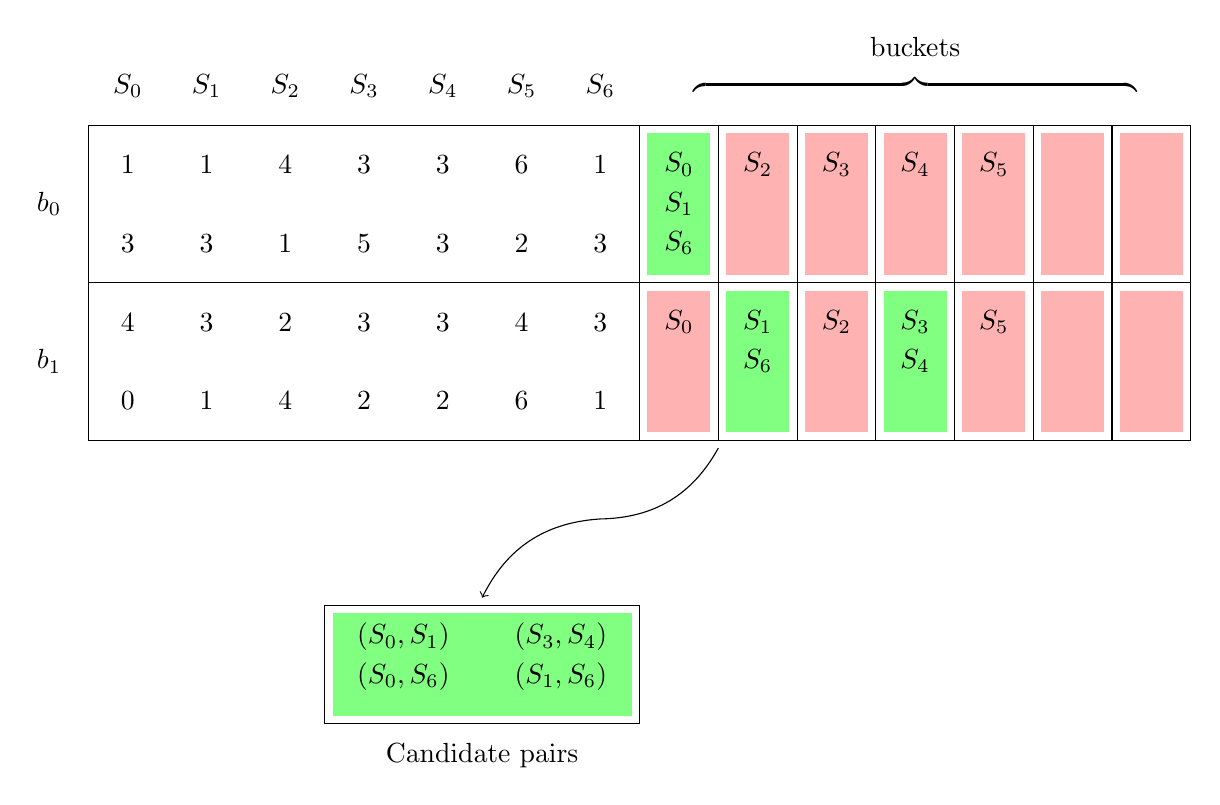
\begin{tikzpicture}
            \draw rectangle (14,4);
            \draw rectangle (7,2);
            \draw (0,2) rectangle (7,2);
            \draw (7,0) rectangle (8,4);

            \foreach \x in {0,...,6} \draw (\x+7, 0) rectangle (\x+7+1, 2);
            \foreach \x in {0,...,6} \draw (\x+7, 2) rectangle (\x+7+1, 4);
            \foreach \x in {0,...,6} \draw (\x+.5, 4.5) node {$S_\x$};

            \draw (-.5,3) node {$b_0$};
            \draw (-.5,1) node {$b_1$};

            % The overbrace
            \draw (10.5, 4.5) node {$\overbrace{\qquad\qquad\qquad\qquad\qquad\qquad\qquad\qquad}$};
            \draw (10.5,5.0) node {buckets};

            % Signature matrix (left part)
            \draw (0.5,3.5) node {1};
            \draw (0.5,2.5) node {3};
            \draw (0.5,1.5) node {4};
            \draw (0.5,0.5) node {0};

            \draw (1.5,3.5) node {1};
            \draw (1.5,2.5) node {3};
            \draw (1.5,1.5) node {3};
            \draw (1.5,0.5) node {1};

            \draw (2.5,3.5) node {4};
            \draw (2.5,2.5) node {1};
            \draw (2.5,1.5) node {2};
            \draw (2.5,0.5) node {4};

            \draw (3.5,3.5) node {3};
            \draw (3.5,2.5) node {5};
            \draw (3.5,1.5) node {3};
            \draw (3.5,0.5) node {2};

            \draw (4.5,3.5) node {3};
            \draw (4.5,2.5) node {3};
            \draw (4.5,1.5) node {3};
            \draw (4.5,0.5) node {2};

            \draw (5.5,3.5) node {6};
            \draw (5.5,2.5) node {2};
            \draw (5.5,1.5) node {4};
            \draw (5.5,0.5) node {6};

            \draw (6.5,3.5) node {1};
            \draw (6.5,2.5) node {3};
            \draw (6.5,1.5) node {3};
            \draw (6.5,0.5) node {1};

            % Fill all with red (in right part)
            \foreach \x in {0,...,6} \path[fill=red!30] (7.1+\x,0.1) rectangle (7.9+\x,1.9);
            \foreach \x in {0,...,6} \path[fill=red!30] (7.1+\x,2.1) rectangle (7.9+\x,3.9);

            % Fill the right ones with green
            \path[fill=green!50] (7.1,2.1) rectangle (7.9,3.9);
            \path[fill=green!50] (8.1,0.1) rectangle (8.9,1.9);
            \path[fill=green!50] (10.1,0.1) rectangle (10.9,1.9);

            % Names
            \draw (7.5,3.5) node {$S_0$};
            \draw (7.5,3.0) node {$S_1$};
            \draw (7.5,2.5) node {$S_6$};
            \draw (8.5,3.5) node {$S_2$};
            \draw (9.5,3.5) node {$S_3$};
            \draw (10.5,3.5) node {$S_4$};
            \draw (11.5,3.5) node {$S_5$};

            \draw (7.5,1.5) node {$S_0$};
            \draw (8.5,1.5) node {$S_1$};
            \draw (8.5,1.0) node {$S_6$};
            \draw (9.5,1.5) node {$S_2$};
            \draw (10.5,1.5) node {$S_3$};
            \draw (10.5,1.0) node {$S_4$};
            \draw (11.5,1.5) node {$S_5$};


            % Arrows
            \path[-] (8,-.1) edge [bend left] (6.5,-1);
            \path[->] (6.5,-1) edge [bend right] (5,-2);

            % Candidate squares
            \path[fill=green!50] (3.1, -3.5) rectangle (6.9, -2.2);
            \draw (3,-3.6) rectangle (7,-2.1);

            % Candidate signatures
            \draw (4,-2.5) node {$(S_0, S_1)$};
            \draw (4,-3.0) node {$(S_0, S_6)$};
            \draw (6,-3.0) node {$(S_1, S_6)$};
            \draw (6,-2.5) node {$(S_3, S_4)$};

            \draw (5,-4.0) node {Candidate pairs};
            

        \end{tikzpicture}
    \caption{LSH buckets and bands}
    \label{fig:lsh_buckets}
    \end{center}
\end{figure}


% Example of algorithm
\begin{center}   
    \captionof{algorithm}{Locality Sensitive Hashing algorithm}\label{alg:lsh}
    \begin{algorithmic}
    
    \BState \textbf{Calculate signature matrix as in algorithm \ref{alg:minhashing}}\\

    \State $SIG\gets \text{signature matrix}$
    \State $S\gets \text{number of signatures}$
    \State $bucket\_list\gets \text{empty list}$
    \State $B\gets \text{number of bands}$\\

    \BState \emph{Fill the buckets}
    \For{$b_i$ in $i = 0 \ldots B-1$}
        \State $h_i \gets \text{empty dictionary}$
        \State $bucket\_list.append(h_i)$
        \For{$SIG_j[b_i]$ in $j = 0 \ldots S-1$}
            \State $key \gets SIG_j[b_i]$
            \If{$key$ in $h_i$}
                \State $bucket \gets h_i[key]$
            \Else
                \State $bucket \gets \text{empty list}$
            \EndIf
            \State $bucket.append(j)$
        \EndFor
    \EndFor\\

    \State $candidate\_pairs \gets \text{empty set}$
    \ForAll{$h_i$ in $bucket\_list$}
        \ForAll{$key$ in $h_i$}
            \State $bucket \gets h_i[key]$
            \If{$bucket.length > 1$}
                \For{$pair$ in $bucket$}
                    \State $candidate\_pairs.add(pair)$ 
                \EndFor
            \EndIf
        \EndFor        
    \EndFor\\

    \BState \textbf{Calculate similarities from signature matrix as in algorithm \ref{alg:minhashing}, for the candidate pairs.}

    \end{algorithmic}
\end{center}


% Example of a gnuplot input
\begin{figure}[H]
    \begin{center}
        \input{plots/scurve.tex}
        \caption{S-curve - $f(s) = 1 - (1 - s^r)^b$ ; $k = 1000$}
        \label{fig:scurve}
    \end{center}
\end{figure}


% Example of a table
\begin{figure}[H]
    \begin{center}
        \begin{tabular}{c|c|c}
              & Actual & LSH \\
            \hline
            1 & 1.0 & 1.0 \\
            2 & 1.0  & 1.0 \\
            3 & 0.667 & 0.702 \\
            4 & 0.667 & 0.695 \\
            5 & 0.667 & 0.689 \\
            6 & 0.667 & 0.684 \\
            7 & 0.667 & 0.681 \\
            8 & 0.667 & 0.681 \\
            9 & 0.667 & 0.677 \\
            10 & 0.667 & 0.673 
        \end{tabular}
        \caption{Correctness of LSH}
        \label{tab:lsh-correctness}
    \end{center}
\end{figure}


% Example of equation
\begin{equation}
    \frac{B(64;R,r_1,r_2)}{B(1;R,r_1,r_2} \Rightarrow \frac{64 R}{R + 1 - r_1}
    \label{eq:improvementratio}
\end{equation}


% Example of graphic
\begin{figure}[H]
    \begin{center}
        \includegraphics{plots/bbit/bbit.eps}
        \caption{b-Bit storage improvement}
        \label{fig:bbit}
    \end{center}
\end{figure}
